%%%%%%%%%%%%%%%%%%%%%%%%%%%%%%%%%%%%%%%%%%%
%
% Template for Final Year Projects
%
\documentclass[12pt,a4paper]{amsart}

\usepackage{amsmath}
\usepackage{amsthm}

\usepackage{enumerate}
%\usepackage{amsrefs}

\usepackage{tikz}
\usepackage{subfig}
\usepackage{graphicx}

\usepackage{pgfplots}

\usepackage{texdraw}

\usepackage{biblatex}
\addbibresource{main.bib}

\newcommand{\trop}[1]{\operatorname{trop}(#1)}
\newcommand{\val}[1]{\operatorname{val}(#1)}
\newcommand{\Gval}{\Gamma_{\operatorname{val}}}
\newcommand{\init}[2]{\operatorname{in}_{#1}(#2)}
\newcommand{\initw}[1]{\init{w}{#1}}
\newcommand{\st}[2]{#1\cap_{st} #2}

\newcommand{\N}{\mathbb{N}}
\newcommand{\Z}{\mathbb{Z}}
\newcommand{\Q}{\mathbb{Q}}
\newcommand{\R}{\mathbb{R}}
\newcommand{\C}{\mathbb{C}}

\newcommand{\T}{\mathbb{T}}
\newcommand{\TM}{\mathcal{M}}
\newcommand{\TN}{\mathcal{N}}

\newcommand{\K}{K}

\newcommand{\cont}{\text{\textreferencemark}}

\newtheorem{thm}{Theorem}[section]
\newtheorem{cor}{Corollary}[thm]
\newtheorem{lem}[thm]{Lemma}

\theoremstyle{definition}
\newtheorem{defn}{Definition}[section]
\newtheorem{ex}{Example}[section]

\theoremstyle{remark}
\newtheorem*{rem}{Remark}
\newtheorem*{note}{Note}
\newtheorem{case}{Case}


\begin{document}


%%%%%%%%%%%%%%%%%%%%%%%%%%%%%%%%%%%%%%%%%%%
%
% Topmatter
%
\title{Tropical Geometry and the Automata}
\author{James Grant Dolan}
\begin{abstract}
Tropical Geometry is a variant of Algebraic Geometry that began its consolidation in the late 20th Century. The initial motivation for the definition of Tropical Geometry was for its application within the field of Automata Theory. I will outline the historical origins of the subject and introduce the key mathematicians involved in the continued development of the area. In recent years it has been applied in dynamic programming to economics. This paper will focus on Tropical Geometry as it relates to Automata Theory. I will look at historical and contemporary work in forging the connection between the fields and show how this connection has evolved.
\end{abstract}
\maketitle
%
%
%%%%%%%%%%%%%%%%%%%%%%%%%%%%%%%%%%%%%%%%%%%

%%%%%%%%%%%%%%%%%%%%%%%%%%%%%%%%%%%%%%%%%%%
%
% Main body of the document
%

\tableofcontents

\newpage
\section*{Introduction}

Tropical Geometry is a variant of Algebraic Geometry that began its consolidation in the late 20th Century.
Though the basic ideas of tropical analysis have been formulated independently across many areas of mathematics for some time, it was only then that the ground work was laid for the topic and indeed it was attributed its unique name.
It was so named in honour of computer scientist Imre Simon, who contributed massively to the field\cite{10.1007/BFb0017135}, in reference to the tropical climate of his native Brazil and the relatively unexplored nature of the field.

\subsection*{Past}
In this paper I will outline the historical origins of the subject and introduce the key mathematicians involved in the continued development of the area, with reference to specific key works.
In doing so I will build up a common knowledge base reflecting the current state of the field.
This will include a variety of sources from various areas of mathematics with varying strengths and weaknesses.
\subsection*{Present}
I will then go on to give an understanding of the applications of Tropical Geometry and show how the scope of the tools contained within have grown across time.
\subsection*{Future}
Next, I will give an overview of the latest developments within the field and possible directions that could be further explored in future. 
Finally, I will delve into the most recent works as they relate to Automata Theory and expand upon the already understood relations.

In one of the earliest papers on the topic\cite{10.1007/BFb0017135} Imre Simon talks about the Tropical semiring with respect to automata theory and the motivations behind its discovery in the field.
For an understanding of the sum of early work see \textit{Tropical Semirings}\cite{pin1998tropical} by Jean-Eric Pin, another key contributor to the field.
The survey is written from the computer science perspective and as such takes the time to introduces mathematical objects, such as monoids and semirings, that a reader, coming from the school of mathematics, may very well already be familiar.
This however proves to maximise the work's accessibility and makes it a great entry point into Tropical Geometry.
The book proves an interesting read not only for its exploration of the immediate applications of Tropical Geometry but also for a slightly different perspective on its definition and construction.

\newpage
\section{Foundation}
In this section we lay out the foundation of tropical geometry with the goal of explaining the fundamental theorem of tropical geometry and the structure theorem.
By the fundamental theorem, we found alternate ways to define the tropicalization of a variety for use in both the construction of these tropical tropicalizations and proofs about their properties.
Juxtaposed to this, the structure theorem gives us a more philosophical understanding of the relation between polyhedral and tropical geometry.

For a more complete view of the subject see \textit{Introduction to Tropical Geometry}\cite{MaclaganDiane1974-author2015Ittg} by Maclagan and Sturmfels, the current authorities on the subject. More recently, Sturmfels produced a lecture series\cite{12Trop} for the Max Planck Institute, of which he is the director, that serve as a very good accompaniment to the book.

This book itself introduces Tropical Geometry as a ``combinatorial shadow" of algebraic geometry so a basic understanding of algebraic geometry is required to gain  a full appreciation of the text and indeed the field as a whole.
To this end, \textit{Ideals, Varieties, and Algorithms}\cite{CoxDavid2007IVaA} by Cox, Little, and O’Shea is also recommended. The book goes over algebraic geometry in a way that is accessible to undergraduate students.
For a more complex understanding of Tropical Geometry see \textit{Nonarchimedean and tropical geometry}\cite{baker2016nonarchimedean} by Matthew Baker and Sam Payne.

Maclagan and Sturmfels were motivated to produce their book by the recent increase in interest in the subject among the mathematics community brought on by advancements in computing power allowing a greater insight into combinatorial mathematics as a whole. The writers hoped this would aid the move of the subject to undergraduate teaching.

It is also recommended you carry some reference texts on polyhedra and polytopes.
For this purpose \textit{Lectures on Polytopes}\cite{ZieglerGunterM1995Lop} by Ziegler would make excellent companion reading. This book will aid in gaining an intuition regarding the structures generated by the geometries discussed later in the paper.

\subsection{The Tropical Semiring}
\subsubsection{Definition}
For purposes that will become apparent later, we would like to obtain a semiring in the operations $\min, +$, that is the minimum operator together with standard addition. Note, it is clear that we may not obtain a ring by these two operations as $\min$ is an inherently 'lossy' operation, meaning information is always lost about the operands, and thus it can have no general inverse. We would also like this semiring to act over a set similar to the reals. While the reals themselves give us a unit in the standard additive identity, $0$, we do not however get a zero in the reals, that is an identity under $\min$ that is also immutable under addition. To obtain this we must adjoin an additional element to our set that is defined in this way. It is convenient to denote such an element with $\infty$ as on a bounded subset of $\R$ these properties would hold for any arbitrarily large number. With this notation, we can rewrite the above conditions as follows;
\begin{equation}
    \begin{aligned}
        \min(\infty, a) = a,\quad \infty + a = \infty&\quad\forall\quad a\in\R \\
        \min(\infty, \infty) = \infty,\quad \infty + \infty = \infty&.
    \end{aligned}
\end{equation}
We can see from this that this element behaves much as would be expected of infinity.

\begin{defn}
We can denote the above constructed semiring by $(\R\cup\{\infty\},\min,+)$ and call it the \textbf{Tropical Semiring}. Equivalently, using a more specific notation, we can write $(\T,\oplus,\otimes)$ with the individual notation in this tuple representing the \textbf{Real Tropical Numbers}, \textbf{Tropical Addition} and \textbf{Tropical Multiplication} respectively.
\end{defn}

It is worth noting that if we could have instead constructed our semiring using the $\max$ operation in place of $\min$ in which case the appended element would instead behave as $-\infty$. In fact, these two rings would be isomorphic under negation so this alternative notation makes sense. We could have also tried to construct this semiring over the integers or indeed the natural numbers. These would also form valid semirings with just the addition of the infinity element as defined before. We will touch on these later subsemirings later but for now we work exclusively over the real tropical numbers.
% We call these the discrete tropical semiring and the non-negative discrete tropical semiring respectively.

%\subsubsection{First Applications}
\subsection{Tropicalization of Polynomials}

\subsubsection{Tropical Polynomials}

To define the tropicalization of polynomials we must first describe what these so called 'tropical' polynomials should look like. Ideally, we should want them take much the same form as the classical polynomials. That is to say a tropical polynomial over some field $\K$ in $n$ variables takes the form
\begin{equation}
    p(x_1,\dots,x_n) = \bigoplus_{i=0}^m a_i\bigotimes_{j=1}^n x_j^{\otimes b_{ij}}
\end{equation}
for some $m\in\N$, $a\in\T^m$, $b\in \N^{m\times n}$ with distinct columns. This is simply the definition of the classical polynomial with the classical operations substituted out for our new tropical ones.

To examine the structure of this object, let us first consider a tropical polynomial in just one variable.
\begin{ex}
Take a general tropical polynomial in one term, using the above, it can be written in the form
\begin{equation}
    p(x) = \bigoplus_{i=0}^m a_i\otimes x^{\otimes b_{i}}
\end{equation}
For some  $m\in\N$, $a\in\R^m$, $b\in \N^m$
\begin{note}
Here, we restrict $a$ to the reals as any term with coefficient $\infty$ will not contribute to the polynomial.
\end{note}
In fact, by leveraging the uniqueness of each element in $b$, we can reorder the monomials and rewrite $p(x)$ in a more familiar way by
\begin{equation}
    p(x) = \bigoplus_{i=0}^N \hat{a}_i\otimes x^{\otimes i}
\end{equation}
for some $N\geq m$ with $\hat{a}_i$ defined as $a_j$ if $b_j = i$ for some $0\leq j\leq m$ and $a_j=\infty$ otherwise. Another way of stating this is to say $\hat{a_i}$ is the coefficient of $x^{\otimes i}$ if it appears in the polynomial and the zero of our semiring, $\infty$, otherwise to offset its inclusion in the sum.

Finally, we can make sense of this by rewriting this polynomial using classical notation as
\begin{equation}
    p(x) = \min_{0\leq i\leq N} \{\hat{a}_i + ix\}.
\end{equation}
As desired, we see that if we have some finite element in $\hat{a}$, i.e. we do not have the zero polynomial, we can choose such a term with this coefficient and guarantee that it will be lesser than any term with coefficient $\infty$ thus justifying our implicit assumption that these terms do not contribute to the overall polynomial.

From this we may propose that such a polynomial will be piecewise linear. It should also be continuous as, at finitely many critical points were one linear term subducts another, both must take the same value. Given the fact there are finitely many terms, we can therefore deduce that there will be finitely many such intersections and there are finitely many linear pieces to the polynomial.

%It is also smooth at all but finitely many points where the endpoints of the line segments join. We can tell that the function is monotonically increasing as each term in the tropical sum (min) is monotonically increasing.
\end{ex}

We can go further than this and examine such a polynomials behaviour with defined degree and coefficients.
\begin{ex}
Take the tropical polynomial
\begin{equation}
    \hat{p}(x) = 11\oplus4\otimes x\oplus1\otimes x^2 = 11\oplus4x\oplus1x^2
\end{equation}
Again, to aid our intuition, let us rewrite this using classical notation.
\begin{equation}
    \hat{p}(x) = \min\{11,4+x,1+2x\}
\end{equation}
Given these concrete values, can now plot this polynomial on a graph to see if it agrees with our initial expectations as has been done below in Figure \ref{fig:poly}.
\begin{figure}[h]
\centering
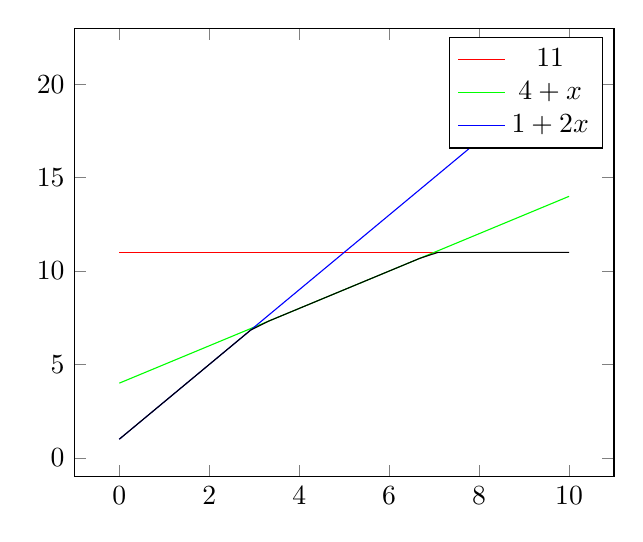
\begin{tikzpicture}[domain=0:10]

\begin{axis}
\addplot[draw=red]{11};
\addlegendentry{$11$}
\addplot[draw=green]{4+x};
\addlegendentry{$4+x$}
\addplot[draw=blue]{1+2*x};
\addlegendentry{$1+2x$}
\addplot[draw=black]{min(11,4+x,1+2*x)};
\end{axis}

\end{tikzpicture}
\caption{A plot of $\hat{p}(x) = \min\{11,4+x,1+2x\}$}
\label{fig:poly}
\end{figure}

As you can see Figure \ref{fig:poly} very much agrees with what was expected of such a graph. There are three distinct linear segments of the line with each corresponding to one of the linear terms. It is worth noting that this is not always guaranteed to be the case as if we substituted the middle term of this polynomial with $15\otimes x$, from the graph it is clear to see that this would never attain the minimum value and would always be subseded by one of the other terms leading to two distinct linear segments in the graph.
\end{ex}

We notice that the above example also has the distinct property that each successive line segment is of a strictly shallower gradient. In fact, by peaking ahead we see this property holds for many more polynomials such as those described by Figure \ref{fig:roots}. However, we would like a more geometric analogue for this property and as such this leads us to introduce the definition of a concave function.

%Rather than talking about the gradient of a tropical polynomial it is far more useful to describe the polynomial geometrically. More specifically it is far easier to describe the graph of the polynomial in higher dimensions as concave.
\begin{defn}[Concave]\label{def:concave}
we cay that a function $f:\R^n\to\R$ is \textbf{concave} if for all $x,y\in\R^n$ we have that
\begin{equation}\label{eq:concave}
    f\left(\frac{x+y}{2}\right) \geq \frac{f(x) + f(y)}{2}.
\end{equation}
\end{defn}

\begin{note}
This may also be referred to as \textbf{concave down} in some textbooks with the complementary \textbf{concave up} referring to such a function where the inequality \eqref{eq:concave} is inverted.
\end{note}

We see that for the above definition the shape described by the region under a concave function will itself always be concave thus motivating this description of such a function. In fact, not only are the properties divulged so far good descriptors of tropical polynomials we can see below that they can be used to entirely redefine the tropical polynomials in terms of these properties.

\begin{lem}
The tropical polynomials correspond exactly to the piecewise-linear concave functions on $\R^n$ with integer coefficients.
\end{lem}
\begin{proof}
It has already been shown above that every tropical polynomial has a corresponding piecewise-linear functions with the required properties.
\end{proof}

Following on from this, we would also want to equip these polynomials with some notion of a root mirroring that of a root in classical algebra. Now, in classical algebra we define the roots of a polynomial $p:A^n\to K$ as exactly those elements $a_i\in A^n$ where $p(a_i)=0_K$. If we are to use this definition for our tropical polynomials we would be finding elements $a_i\in\T^n$ where $p(a_i)=\infty$.
Unfortunately, this definition is not very interesting as apart from the trivial tropical polynomial, where the polynomial is $\infty$ everywhere, every tropical polynomial is finite so the roots of a polynomial under this definition would either be the empty set of the whole of the domain.

Now, there is an alternative definition of the roots of a polynomial that does not rely on the function zeros and that is the factorisation definition that is we say that $a_i$ is a root of some polynomial $p:A^n\to K$ if and only if we can write
\begin{equation}
    p(x) = (x - a_i)q(x)
\end{equation}
for some other polynomial $q:A^n\to K$. Seeing how in the tropical semiring we have no additive inverse we write the following closely related definition.

\begin{defn}
We say that $a_i$ is a \textbf{tropical root} of some function $p:\T^n\to \T$ if we have
\begin{equation}
    p(x) = (x \oplus a_i)^{\otimes k}\otimes q(x)
\end{equation}
for some $k\in\N$, polynomial $q:A^n\to K$. In fact, if $k$ is maximal under choice of all $q$ we say that $a_i$ is a root of \textbf{degree} $k$. We also call the sum $(x \oplus a_i)$ a \textbf{tropical factor} of the polynomial
\end{defn}

\begin{ex}\label{ex:roots}
Take the polynomials $p_1(x) = 1 \oplus x$, $p_2(x)=1\oplus 2x$, $p_3(x)=1\oplus x\oplus 2x$ graphed below in Figure \ref{fig:roots}. In the first polynomial we can simply read off the only root $x=1$ where $q_1(x) = 0$. Notice this also describes the intersection of the two lines that make up the polynomial. Similarly the root of $p_2$ is $x=1/2$. This also happens to be an intersection point of the two lines. However, in the more complex case of $p_3$ we see that the only two roots are $x=0$ and $x=1$ and this only accounts for two of the three possible intersection points. Note, however, that these are exactly the intersection points that actually take place on the tropical polynomial.
\end{ex}

\begin{figure}[h]
\centering
    \subfloat[$p_1(x) = 1 \oplus x$]{
        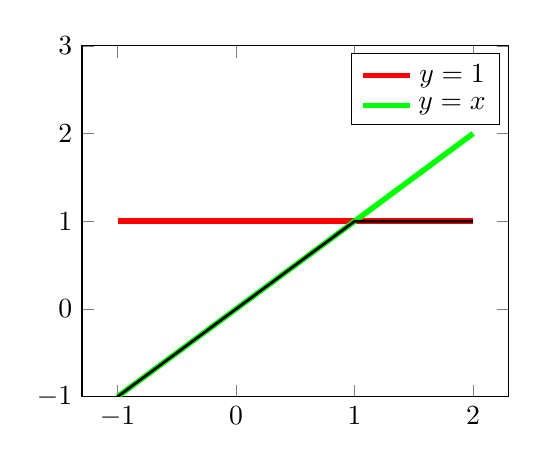
\begin{tikzpicture}[domain=-1:2]
        
            \begin{axis}[width=7cm,ymin=-1,ymax=3]
            \addplot[draw=red,line width=2pt]{1};
            \addlegendentry{$y=1$}
            \addplot[draw=green,line width=2pt]{x};
            \addlegendentry{$y=x$}
            \addplot[draw=black,line width=1pt]{min(1,x)};
            \end{axis}
        
        \end{tikzpicture}
    }
    \subfloat[$p_2(x)=1\oplus 2x$]{
        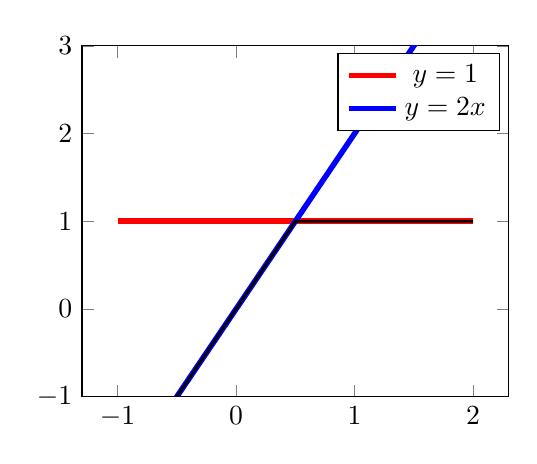
\begin{tikzpicture}[domain=-1:2]
        
        \begin{axis}[width=7cm,ymin=-1,ymax=3]
        \addplot[draw=red,line width=2pt]{1};
        \addlegendentry{$y=1$}
        \addplot[draw=blue,line width=2pt]{2*x};
        \addlegendentry{$y=2x$}
        \addplot[draw=black,line width=1pt]{min(1,2*x)};
        \end{axis}
        
        \end{tikzpicture}
    }
    
    \subfloat[$p_3(x)=1\oplus x\oplus 2x$]{
        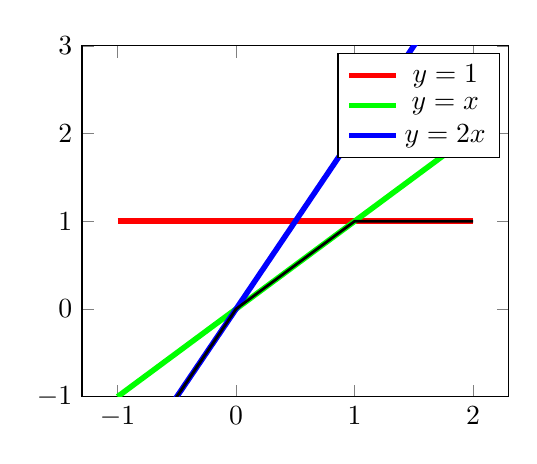
\begin{tikzpicture}[domain=-1:2]
        
        \begin{axis}[width=7cm,ymin=-1,ymax=3]
        \addplot[draw=red,line width=2pt]{1};
        \addlegendentry{$y=1$}
        \addplot[draw=green,line width=2pt]{x};
        \addlegendentry{$y=x$}
        \addplot[draw=blue,line width=2pt]{2*x};
        \addlegendentry{$y=2x$}
        \addplot[draw=black,line width=1pt]{min(1,x,2*x)};
        \end{axis}
        
        \end{tikzpicture}
    }
\caption{Various functions and their roots}
\label{fig:roots}
\end{figure}

The above example motivates an equivalent definition of the root of a tropical polynomial as the intersection of these such lines.

\begin{lem}
The roots of a tropical polynomial are exactly the points where the minimum is attained at least twice.
\end{lem}

\begin{note}
This is equivalent to our above description in Example \ref{ex:roots} as the fact that the minimum is attained twice means this must lie at the intersection of two lines that make up the tropical polynomial. However, the fact that the minimum is actually attained here necessitates that this intersection actually appear on the tropical polynomial.
\end{note}

It is convenient to have a notion of how we can represent a tropical polynomial a as a classical polynomial. First we need a way to modify the coefficients in a way that maps the identities in one semiring to another so valid classical polynomials are mapped to valid tropical polynomials.
\newpage
\subsubsection{Valuation Maps}
\begin{defn}[Valuation Map]
For a field $\K$, we call a function $v:\K\to\T$ a \textbf{valuation map} over the field $\K$, or more simply just a \textbf{valuation} over $\K$, provided it satisfies the following conditions;
\begin{enumerate}
    \item $\val{x} = \infty$ if and only if $x = 0$
    \item $\val{xy} = \val{x} + \val{y}$
    \item $\val{x+y} \geq \min( \val{x},\val{y} )$
\end{enumerate} for all $x,y\in \K^*$.
We call the additive subgroup over the image of a valuation map it's \textbf{value group} and it is denoted $\Gval\subseteq\R$.
\end{defn}

\begin{note}
We can assume without loss of generality that a general valuation group is contains $1$ as $\lambda\cdot v$ is a valuation for all valuation $v$, $\lambda\in\R^+$
\end{note}

Now the above are only the necessary properties for a such a function to be a valuation map. There are a handful of other useful properties of all valuations induced by these simple rules that it is (diligent) to take note of for use in larger and more complex proofs.

\begin{lem}
Any valuation $v$ over a field $\K$ has the following additional properties;
\begin{enumerate}
    \item $\val{1} = \val{-1} = 0$
    \item $\val{-x} = \val{x}$
    \item $\val{x^{-1}} = -\val{x}$
    \item If $\val{x} \neq \val{y}$ then condition (3) above is a strict equality.
\end{enumerate} for all $x,y\in \K^*$
\end{lem}
\begin{proof}
By condition (1) we have
\begin{align*}
    \val{1} = \val{1\cdot1} = 2\val{1}\quad&\implies\quad \val{1} = 0\\
    \val{1} = \val{-1\cdot-1} = 2\val{-1}\quad&\implies\quad \val{-1} = \val{1} = 0
\end{align*}
thus proving property (1).
Following on from this we also have
\begin{align*}
    \val{-x} = \val{-1\cdot x} = \val{-1} + \val{x} = \val{x}
\end{align*}
thus proving property (2).
\begin{align*}
    \val{1} = \val{x\cdot x^{-1}} = \val{x} + \val{x^{-1}}\quad&\implies\quad \val{x^{-1}} = -\val{x}
\end{align*}
thus proving property (3).

In order to prove the final property, we will assume, without loss of generality, that $\val{a}<\val{b}$ so that
\begin{align*}
    \val{a}&\geq \min(\val{a+b},\val{-b})
    \intertext{by property (2) we have}
    \val{a}&\geq \min(\val{a+b},\val{b})
    \intertext{and as $\val{b}>\val{a}$}
    \val{a}&\geq \val{a+b}.
    \intertext{Together with condition (3) we get}
    \val{a+b} &= \val{a} = \min( \val{a},\val{b} )
\end{align*}

\end{proof}

\begin{ex}[The p-adic valuation]
Take the field of rational numbers $\Q$ and any prime number $p$. We can define a valuation $v_p:\Q\to\T$ by $v_p(p)=1$, $p_k(q) = 0$ for all $q\in\Z^*$ coprime with respect to $p$. This completely defines $v_p$ on $\Q$ under the assertion that this be a valuation as we define $p_k(0) = \infty$ by condition (1) and any other undefined element in $\Q$ can be written as a product of the well defined elements $p, a/b\in\Q$ and be evaluated using condition (2).

To show that condition (2) is completely satisfied we must show that it also holds when $x$ and $y$ are of different 'type'.
\begin{case}
$x = p^k$, $y = p^l$
\begin{align*}
    \val{x} + \val{y} &= \val{p^k} + \val{p^l}\\
    &= k+l = \val{p^{k+l}}\\
    &= \val{p^k p^l} = \val{xy}
\end{align*}
\end{case}
\begin{case}
$x = a/b$, $y = c/d$
\begin{align*}
    \val{x} + \val{y} &= v\left(\frac{a}{b}\right) + v\left(\frac{c}{d}\right) = 0\\
    &= v\left(\frac{ac}{bd}\right) = v\left(\frac{a}{b}\frac{c}{d}\right) = 
    \val{xy}
\end{align*}
\end{case}
\end{ex}

%For the remainder of this paper we shall use $K = \K\{\{t\}\}$ to denote the general Piuseux field over the general field $\K$

\begin{thm}\label{thm:PuiseuxClosed}
For any algebraically closed field of characteristic zero, the field of Puiseux series over that filed will also be algebraically closed.
\end{thm}

\begin{ex}[The Puiseux valuation]
Take the field of complex Puiseux series $\C\{\{ t \}\}$. We can define a natural valuation $v$ on this field by taking every $c(t)\in\C\{\{ t \}\}^*$ to the lowest power on $t$ in the unique Laurent series expansion of $c(t)$ i.e. the unique $k\in\T$ such that $c(t) = a t^k + o(t^k)$ for some $\C$. We can say this is unique as if this were true for some $k,l\in\T$, $k\leq l$ without loss of generality, then we have
\begin{align*}
    a t^k + o(t^k) = b t^l + o(t^l) = bt^l + o(t^k)\quad\implies\quad k = l\text{ and }a = b
\end{align*}
Now in actual fact what this valuation is telling us about each of these elements, which you could perhaps guess by the use of Laurent series and little-o notation, is their behaviour at and about the point point $t=0$. More specifically, it encodes both weather there is a zero or a pole at this point, by way of the sign of the valuation, and the order of such a feature, by way of the magnitude of the valuation. Of course should the function have zero valuation there is neither a zero or a pole at this point.

This notion can also be extended to the rational functions $\C(t)\subset \C\{\{ t \}\}$ evaluating each functions unique Laurent series expansion instead of directly evaluating the function. For example given
\begin{align*}
    c(t) &= \frac{8t^3+2t^4+4t^5}{5t+9t^3}
    \intertext{we can compute the Laurent series and find}
    c(t) &= \frac{8t^2}{5} + \frac{2t^3}{5} - \frac{52t^4}{25} + O(t^5)
    \intertext{and now all that remains is to evaluate the series as before}
    &= \frac{8}{5}t^2 + o(t^2)\implies \val{c(t)}=2
\end{align*}

By \ref{thm:PuiseuxClosed} we can also say that the Puiseux series $\C\{\{ t \}\}$ is closed and thus induces the inclusion $\overline{\C(t)}\hookrightarrow\C\{\{ t \}\}$.
\end{ex}

\subsubsection{Tropicalization}

\defn{Tropicalization}
Take a standard polynomial $f\in\R[x]$, the \textbf{tropicalization} of this polynomial is obtained by substitution of multiplication and addition by their tropical counterparts and the coefficients by their tropical evaluation. That is given polynomial $f = \sum_{i=0}^n c_ix^i$, and valuation $v$, we have
\begin{equation}
    \trop{f} = \bigoplus_{i=0}^n \val{c_i} \otimes \underbrace{x\otimes\dots\otimes x}_\text{$i$ times}.
\end{equation}
Proper notation for tropical indices is
\begin{equation}
    x^{\otimes n} = \underbrace{x\otimes\dots\otimes x}_\text{$n$ times}
\end{equation}
however, as with tropical multiplication, where there is no ambiguity we can drop the $\otimes$ and represent this with a standard index.

\begin{defn}[Laurent field]
A \textbf{Laurent series} is a power series that allows a finite number of negative exponents.
The \textbf{Laurent field} over some field $\K$ is thus the field containing all such series with coefficients in $\K$. We denote this field $\K((t))$ where $t$ is the indeterminate.
\end{defn}

\begin{ex}
The general elements of the Laurent series $\R((t))$ are of the form
\begin{equation*}
    \sum_{n=N}^\infty c_n t^n
\end{equation*}
for some $N\in\Z$, $c_N,c_{N+1},\dots\in\R$. Note that for certain elements of the series that contain negative exponents exists, $N$ will be negative also.
\end{ex}

\begin{defn}[Puiseux field]
A \textbf{Piuseux series} is a power series that allows both a finite number of negative exponents, and fractional exponents. One additional restriction is that all of the fractional exponents must be able to be expressed over the same denominator.
The \textbf{Puiseux field} over some other field $\K$ is thus the field containing all such series with coefficients in $\K$. We denote this field $\K\{\{t\}\}$ where $t$ is the indeterminate.
\end{defn}

\subsection{Tropical Geometry}

The Tropical Geometry concerns itself with the affine varieties generated by Laurent polynomials over some general field $K$; More specifically, the very affine varieties generated by ideals in the Laurent polynomials. Recall that affine varieties are calculated by
\begin{equation}
    V(f)=\{ a\in A^n : f(a)=0 \}
\end{equation}
for some function $f:A^n\to K$ acting on affine space. This is readily extend to the ideals in $K[x_0,x_1,\dots,x_n]$ by
\begin{equation}
    V(I) = \bigcap_{f\in I} V(f) = \{ a\in A^n : f(a) = 0\text{ for all } f\in I \}
\end{equation}
for some ideal $I\subseteq K[x_0,x_1,\dots,x_n]$. When working over the affine space, it is natural to consider the various sets arising with respect to the Zariski topology wherein a set is closed exactly when it can be written as the variety of some ideal.

For our purposes, it is also convenient to define an inverse of sorts by way of
\begin{equation}
    I(V) = \{ f\in K[x_0,x_1,\dots,x_n] : f(x) = 0\text{ for all }x\in V \}
\end{equation}
defined for some $V\subseteq A^n$.
\begin{note}
While we have that $V = I^{-1}$, $I$ is not a true inverse as $I(V(\emptyset)) = I(A^n) = \{ \boldsymbol{0} \} \neq \emptyset$ and therefore $I \neq V^{-1}$.
\end{note}

%is generated by the function $V:\T[x_1,\dots,x_n]\to 2^\T$ from polynomials in Tropical semiring to a subset of the tropical numbers where the minimum is attained at least twice.

%Within the field we refer to these operations as Tropical addition and Tropical multiplication respectively and they are denoted $\oplus$ and $\otimes$.
The infinity element is added to the the set to ensure the semiring axioms are satisfied, with $\infty$ being the zero of the semiring. 

\subsubsection{Nice Properties}

\begin{defn}[Multiplicity]
Consider the intersection of two line segments with unit direction vectors $(u_1,u_2)$, $(v_1,v_2)$ respectively.
The \textbf{multiplicity} of points of intersection is defined to be
\begin{equation}
    \left|\det
    \begin{pmatrix}
        u_1 & v_1\\
        u_2 & v_2
    \end{pmatrix}
    \right|
\end{equation}
\end{defn}
\begin{note}
If these line segments intersect at more than one point then they must be parallel and thus the multiplicity will be zero.
\end{note}

%Note, this is the same reason that the repeated root in $y=x^3$ does not result in two intersections of the x-axis.

\begin{thm}[Stable Intersection Principle]
Two general curves, $C$ and $D$, of degree $c$ and $d$ respectively in $\R^2$, take $C_{\epsilon}$ and $D_\epsilon$ representing the prior curves under some perturbation proportional to some $\epsilon>0$.
The limit of $C_\epsilon\cap D_\epsilon$ as $\epsilon\to0$ is a well defined multi-set of $c d$ points contained in the intersection $C\cap D$.
\end{thm}

\begin{defn}[Stable Intersection]
The \textbf{stable intersection} of two tropical curves $C$ and $D$ in $\R^n$ is defined to be union of the piecewise intersection of the elements in each curve where the direct sum of the elements are of the same degree as the whole space $\R^n$. More specifically if we denote the stable intersection as $\st{C}{D}$, we say
\begin{equation}
    \st{C}{D} \quad = \bigcup_{\substack{c\in C,\ d\in D \\ dim(c+d)=n}}c\cap d
\end{equation}
\end{defn}

\begin{thm}[Bézout's theorem]
Two general curves, $C$ and $D$, of degree $c$ and $d$ respectively in $\R^2$ have $c d$ many intersection points when counted with multiplicity.
\end{thm}

\begin{cor}
Any two curves, $C$ and $D$, of degree $c$ and $d$ respectively in $\R^2$ have $c d$ many stable intersection points when counted with multiplicity.
\end{cor}

\subsubsection{Smoothness}

We want some sense of 

\begin{defn}[Smooth]
We call a tropical curve \textbf{smooth} if its dual is a \textbf{unimodular triangulation} that is each cell in the dual is a lattice triangle with unit area \textonehalf.
\end{defn}

\subsection{Tropical Curves}

Early theorem, unpublished

\begin{thm}[Kapranov]
Take any Laurent polynomial $f\in K[x_1^{\pm1},\dots,x_n^{\pm1}]$ the following definitions for $\trop{V(f)}$ coincide with the definition given in XYZ.
\begin{enumerate}
    \item $\trop{V(f)} = \overline{\{ w\in\Gval^n : \initw{f}\text{ is not a monomial} \}}$
    \item $\trop{V(f)} = \overline{\{ (\val{x_1},\dots,\val{x_n}) : (x_1,\dots,x_n)\in V(f) \}}$
\end{enumerate}
\end{thm}


\subsection{Tropicalization of Varieties}

\subsubsection{In the Hypersurface}

\begin{defn}[Tropicalization]
We define the \textbf{tropicalization of a variety} $X$ in the algebraic torus $T^n$ as the intersection of all tropical hypersurfaces derived from the laurent polynomials within its generating ideal. That is
\begin{equation}
    \trop{X} = \bigcap_{f\in I(X)} V(\trop{f}) \subseteq \R^n.
\end{equation}
\end{defn}

\begin{thm}
Take two curves $C = \trop{A}$ and $D = \trop{B}$ for some varieties $A,B$. There exists $t\in\T^n$ such that
\begin{equation}
    \trop{A\cap t B} = \st{C}{D}.
\end{equation}
In fact, the set $U\subset \T^n$ of all such $t$ is Zariski open. That is the set of such $t$ where this is not the case can be written as the variety of some ideal in the polynomial ring.
\end{thm}

\begin{cor}
Given a Laurent polynomial $f\in K[\mathbf{x}^{\pm1}]$, if all of its coefficients are of zero value then the tropical hypersurface $\trop{V(f)}$ is the support of an $n-1$ dimensional polyhedral fan in $\R^n$. More specifically, that fan is the $n-1$ skeleton of the normal fan to the Newton polytope of $f$.
\end{cor}

%From this previous definition of the tropicalization of a variety, we can construct two equivalent definitions

%of tropicalization of a variety provides us two alternate definitions which coincide exactly with the first as follows

\subsubsection{The Fundamental Theorem}

\begin{lem}
$X=V(I)\subset\T^n$
\begin{align*}
    \overline{\val{X}}\subseteq\trop{X}\subseteq\{ w\in\R^n : \initw{I} \neq \langle1\rangle> \}
\end{align*}
\end{lem}

\begin{thm}[The Fundamental Theorem of Tropical Geometry]
Given a variety $X$ in the algebraic torus $T^n$ we can also define the tropicalization
\begin{enumerate}
    \item $\trop{X} = \overline{\{ w\in\R^n : \text{in}_wI(X) \neq (1) \}}$
    \item $\trop{X} = \overline{\{ (\val{x_1},\dots,\val{x_n}) : (x_1,\dots,x_n)\in X \}}$
\end{enumerate}
\end{thm}

\begin{proof}
To prove these sets are equal we shall prove that there is a cyclic chain of inclusions in the sets.

First, we shall prove that $(1)\subseteq\trop{X}$.

\noindent Take $v = (y_1,\dots,y_n)\in\overline{\{ (\val{x_1},\dots,\val{x_n}) : (x_1,\dots,x_n)\in X \}}$ for some variety $X$. We can find $u = (x_1,\dots,x_n)\in X$ such that $\val{x_i} = y_i$ for all $1\leq i\leq n$. We also have that $f(u) = 0$ for all $f\in I(X)$. By \textbf{XYZ} we have $V\in\trop{V(f)}$ for all $f\in I(X)$ and thus $V\in \trop{X}$. This gives us the required inclusion.

Next, we need to prove that $\trop{X}\subseteq(2)$.

\noindent
\end{proof}

\subsection{Structure Theorem}
\begin{thm}[Structure Theorem]
The tropicalization of an irreducible subvariety in the algebraic torus $\T^n$ is the support of a balance weighted $\Gval$-rational polyhedral complex pure of the same dimension.
Moreover, that polyhedral complex is connected through co-dimension one.
\end{thm}
%\subsubsection{Work}
%\subsubsection{Proofs}

\newpage
\section{Application}
As discussed previously the initial motivation for the definition of Tropical Geometry was for its application within the field of Automata Theory.
Moreover, given that the early applications of Tropical Geometry were in Automata Theory and computer science more generally.
Although, Tropical Geometry has been “anonymously” used in maths for some time, applications in this area were less developed around its conception. 
In such areas tropicalization was often thought of as the logarithmic function with arbitrarily large base. It was however understood as a process within the scope of its application and not a general operation in its own right.
For example, in thermodynamics, this limit can be understood as the behaviour of photons as temperature reaches absolute-zero.
Another application of Tropical Geometry resides within dynamical programming. Here, after tropicalization of the adjacency matrix, an optimisation problem becomes one of taking the determinant of the matrix under tropical arithmetic which itself becomes the process of taking the permanent, due to the lack of a well defined negation operation within the arithmetic, that is the usual algorithm for finding determinant taking sums instead of differences. This is best illustrated by example.

\begin{ex}
The permanent of a general $2\times2$ matrix can be calculated by the following;
\begin{equation}
\operatorname{perm}\begin{pmatrix}
a & b\\
c & d
\end{pmatrix} = ad + bc
\end{equation}
Likewise, to find the permanent of a general $3\times3$ matrix we would calculate
\begin{multline}
\operatorname{perm}\begin{pmatrix}
a & b & c\\
d & e & f\\
g & h & i
\end{pmatrix}
\begin{aligned}
    &= (a e+b d)i + (a f+c d)h + (b f+c e)g\\
    &= aei + bdi + afh + cdh + bfg + ceg.
\end{aligned}
\end{multline}
\end{ex}

The Geometry also has some very more real world applications.
In the wake of the 2007 global financial crisis, Economist Paul Klemperer was tasked by the Bank of England with developing a bespoke auction system that could better inform government lending in order to provide liquidity to the banks that, at the time, vitally needed it.
As the problem was fundamentally one of resource allocation, it felt natural to use Tropical Geometry in order to tackle this problem. Indeed, he had already become somewhat familiar with the basic principles whilst organising the British third-generation mobile-phone licence auction earlier in 2000\cite{binmore2002biggest}.
Of course then the subject as we know it today was only in its infancy.
To this end, he invented the Product-Mix Auction\cite{klemperer2010product}.
This system allowed the Bank of England to forgo the weeks of arbitration that were necessary during the earlier 3G auction meaning the capitol could enter the economy as soon as possible and aid financial recovery.
For a full understanding of the mathematics see \textit{Understanding preferences:“demand types”, and the existence of equilibrium with indivisibilities}.\cite{baldwin2019understanding} by Elizabeth Baldwin and Paul Klemperer.

\subsection{Automata Theory}
In this section, I will focus on Tropical Geometry as it relates to Automata Theory.
Automata which are state machines that can either accept or reject a set of inputs depending on what state it leaves the machine in.
These range from simple finite state machines to more complex Turing machines which in comparison have a theoretically unlimited memory capacity as they are able to freely read and write from their own instruction queue.
For an understanding of the basics of finite automata I would recommend \textit{Finite Automata}\cite{lawson2003finite} by Mark V Lawson. Most of the more complete textbooks on Automata Theory are written with an assumption of a basic understanding of computer science so the reading individual papers on specific areas is required to gain a full understanding from a mathematical perspective.

Given that applications in Automata Theory formed the basis for many of the early literature regarding Tropical Geometry\cite{simon1978limited}, it is fitting that we return to the field now to investigate the advances now made possible with 21st century technologies and understanding.
Interesting contemporary works in this field include \textit{Automata in groups and dynamics
and induced systems of PDE in
tropical geometry}\cite{kato2014automata} by Tsuyoshi Kato.
Using these preliminary texts as a basis, I will seek to find more contemporary texts on the subject to inform my study.

\subsection{Semiring Applications}
As previously mentioned, Simon's reconstruction of the tropical semiring was motivated by problems from Automata theory. Moreover, he was interested in finding conditions under which languages were limited that is the Kleene star of such a a language can be represented as the union of only finitely many powers of the language. This was a response to the earlier counter-example provided by Golod and Shafarevich which disproved the conjecture at the heart of the Burnside problem. A full general disproof of the conjecture was later provided by Novikov and Adjan. (check history)

\subsubsection{Main Result}
The talk given by Simon represented only a part of a larger body of work working towards answering a larger problem posited by J.A.Brzozowski, following the disproof of Burnside, in an earlier conference. The problem, as Brzozowski stated it reads as follows;
\begin{quote}
    Is it decidable whether for a given regular set $\R$,
    
    \noindent$\R^*=(\lambda\cup\R)^m$ for some integer $m\geq1$?
\end{quote}
The condition on this statement is equivalent to saying that the set is limited and thus can be restated as a theorem by the following;
\begin{thm}
It is recursively decidable whether a given rational subset $L\subseteq A^*$ is limited or not.
\end{thm}
This is not only true, but there is in fact an algorithm for deciding this that leverages the tropical semiring. 

\begin{defn}
For the remainder of this section we use $\TM=\N\cup\infty$ to denote the \textbf{tropical integer semiring} and $\TN = \{ 0,1,\infty \}$ to denote the \textbf{discrete tropical semiring}

Notice that $\TN$ is a homomorphic image of $\TM$. To represent this define the morphism $\psi:M_n(\TM)\to M_n(\TN)$ to be the function that maps each finite positive entry in the matrix to $1$ and does nothing otherwise. That is
\begin{equation}
    \psi(a)_{ij} = \begin{cases}
    1&\text{if } 0 < a_{ij} < \infty\\
    a_{ij}&\text{otherwise}
    \end{cases}
\end{equation}

Conversely we also have the set inclusion $\iota:M_n(\TN)\hookrightarrow M_n(\TM)$.
For convenience we define $\Psi:M_n(\TM)\to M_n(\TM): a\mapsto \iota(\psi(a))$ 
\end{defn}

Find the condition for a rational subset of a free monoid to be limited. 
\begin{note}
Here a rational language is just a regular language i.e. those languages that can be defined by a regular expression using only finite languages, concatenation, union, and the Kleene star operator.
\end{note}
Find a recursive algorithm to decide this
Unable to find a extended algorithm for context free sets
\subsubsection{Burnside}

In its simplest terms, the aforementioned Burnside problem asks whether every torsion group is locally finite.

For us to understand this statement we must first build up an understanding of the terms within.

\begin{defn}
Take some abelian group $A$. The \textbf{torsion group} $A_T$ of $A$ is the subgroup of $A$ containing only the elements of finite order
\end{defn}

\begin{note}
It is important that the group $A$ chosen above is a abelian group as otherwise we have no grantee that $A_T$ forms a subgroup.
\end{note}

\begin{ex}
%$$\vbox{\tabskip0.5em\offinterlineskip
%    \halign{\strut$#$\hfil\ \tabskip1em\vrule&&$#$\hfil\cr
%    ~     & e   & a   & b   & b^2 & b^3 & \dots\cr
%    \noalign{\hrule}\vrule height 12pt width 0pt
%    e     & e   & a   & b   & b^2 & b^3 &      \cr
%    a     & a   & e   & ab  & ab^2& ab^3&      \cr
%    b     & b   & ab  & b^2 & b^3 & b^4 &      \cr
%    b^2   & b^2 & ab^2& b^3 & b^4 & b^5 &      \cr
%    b^3   & c^3 & ab^3& b^4 & b^5 & b^6 &      \cr
%    \vdots& d   &     &     &     &     & \ddots   \cr
%}}$$
Let $A = Z(x)$ be the integers extended by some element $x$ where $x+x=0$. We have that $(A,+)$ is an abelian group. The torsion subgroup $A_T = \{0,x\} \cong \Z/2\Z$ as all integers besides $0$ have infinite order under addition.
\end{ex}

\begin{defn}
Take a semigroup $S$. We say that $S$ is \textbf{locally finite} if for every finite subset $T\subset S$ the subsemigroup generated by $T$ is also finite.
\end{defn}

Shown for torsion groups over complex numbers
Extended to torsion groups of matrices over any field


With all this understood we can state a weaker form of the Burnside problem to be solved.

\begin{thm}\label{thm:Simon1}
Every torsion subsemigroup of $M_n(\hat{\TM})$ is locally finite.
\end{thm}
\begin{note}
Here we are specifically working over the square matrices with entries in tropical integer semiring
\end{note}

To aid in the proof of this theorem we borrow a result from T.C.Brown \cite{brown1969locally}.

\begin{thm}[Brown]\label{thm:Brown}
Take any semigroup $S$. If there exists a semigroup morphism from $S$ into some known locally finite semigroup $T$ where the preimage of the idempotents in $T$ are all locally finite then you can say that the whole of $S$ is also locally finite.
\end{thm}

The proof of this is more complicated and better explained in its introductory text\cite{brown1969locally}.

\begin{defn}
We define the \textbf{delta function} as the function that takes the value of the largest finite element of a tropical matrix. More specifically we define it as $\delta:M_n(\TM)\to\N$ by
\begin{equation}
    \delta(a) = \max(0\cup\{ a_{ij} : 1\leq i,j \leq n, a_{ij}\leq\infty \})
\end{equation}
for some $a\in M_n(\TM)$.

This function can be extended over a set of tropical matrices. We denote this $\Delta:\mathcal{P}(M_n(\TM))\to\TM$ where
\begin{equation}
    \Delta(X) = \sup(0\cup\{ \delta(a) : a\in X \})
\end{equation}
for some $X\subseteq M_n(\TM)$
\end{defn}

\begin{note}
$X\subseteq M_n(\TM)$ is finite if and only if we have that $\Delta(X)<\infty$.
\end{note}

\begin{lem}\label{lem:simon1}
If we take the convention that for $a,b\in M_n(\TM)$, $a\leq b$ if $a_{ij}\leq b_{ij}$ then for all $a,b,c,d\in M_n(\TM), m\in\N^*$ we have the following;
\begin{enumerate}
    \item $a\leq b$ and $c\leq d \implies ac \leq bd$.
    \item $m(ab) = (ma)(mb)$.
    \item $a\leq b \implies \delta(a)\leq \delta(b)$.
    \item $\delta(ma) = m\cdot\delta(a)$.
    \item $\delta(a)\leq m \implies \Psi(a)\leq a\leq m(\Psi(a))$
    \item $\delta(ab)\leq\delta(a)+\delta(b)$
\end{enumerate}
\end{lem}
%\begin{proof}
%(do later)
%\end{proof}

\begin{defn}
semigroup generation $X^+$
\end{defn}

\begin{lem}\label{lem:simon2}
For all $X\subseteq M_n(\TM)$ we have that,
\begin{equation}
    \Delta(\Psi(X)^+)\leq\Delta(X^+)\leq\Delta(X)\cdot\Delta(\Psi(X)^+)
\end{equation}
\end{lem}
%\begin{proof}
%
%\end{proof}

\begin{cor}\label{cor:simon1}
For all finite $X\subseteq M_n(\TM)$, $X^+$ is finite exactly when $\Psi(X)^+$ is finite.
\end{cor}
\begin{proof}
By Lemma \ref{lem:simon2} we immediately have that
\begin{equation*}
    \Delta(\Psi(X)^+)\leq\Delta(X^+)
\end{equation*}
therefore $\Delta(X^+)$ finite implies $\Delta(\Psi(X)^+$ finite.

To get the opposite implication notice that $X\subseteq M_n(\TM)$ implies that $\Delta(X)<\infty$. Likewise, by assuming $\Delta(\Psi(X)^+$ finite,  Lemma \ref{lem:simon2} tells us that
\begin{equation*}
    \Delta(X^+)\leq\Delta(X)\cdot\Delta(\Psi(X)^+)<\infty
\end{equation*}
thus implying $\Delta(X^+)$ finite
\end{proof}

\begin{cor}\label{cor:simon2}
For all matrix $a\in M_n(\TM)$, $a$ is a torsion exactly when $\Psi(a)$ is a torsion.
\end{cor}
\begin{proof}
This is just an extension of corollary \ref{cor:simon1} using the fact that $a$ is a torsion exactly when $\{a\}^+$ is finite.
\end{proof}

Now we have all of the pieces required o tackle the main proof in this section

\begin{proof}[Proof of Theorem \ref{thm:Simon1}]
Let $S$ be a torsion subsemigroup of $M_n(\TM)$, let $T=\psi(S)$, and let $\beta:S\to T$ be the restriction of $\psi$ to $S$. As $T\subseteq M_n(\TN)$ is finite, by Brown's theorem \eqref{thm:Brown} we only need to find that the preimage of every idempotent in $T$ is locally finite. However Corolloary \ref{cor:simon2} says that as $\beta^{-1}e\subseteq\psi^{-1}e$ for all $e\in T$ idempotent, again we need only prove that all idempotents of $T$ are torsions under $\iota$
\end{proof}

%\subsubsection{Decision Problem}
%\subsubsection{Proofs}

\subsection{Sandpile Model}
One more contemporary application of tropical geometry within automata theory is its use in the study of self-organised critical systems\cite{bak1987self, bak1988self}. In particular the study of the sandpile model, an idealised cellular automaton constructed to display SOC behaviour and has remained the archetypal example of such a system, and its extension to a continuous tropical model\cite{kalinin2018self}.

\subsubsection{Classical}
Abstractly, a sandpile model is defined on the intersection of the integral square lattice, $\Z^2$, and some large convex figure in the Euclidean plane. At each point some number of grains of sand are placed and we define $\varphi$ to be the evaluation of this at a given point.

\ex
Consider the 3x3 sandpile model on the set $\Omega=\{0,1,2\}^2$. On this set we define $\varphi:\Omega\to\N$ to be the function which evaluates the number of grains at each vertex in $\Omega$.

\defn
We say that a vertex, $(x,y)\in\Omega$ is \textbf{unstable} whenever $\varphi(x,y) \geq 4$; otherwise we say that it is \textbf{stable}. We say that a state, $\varphi$, is \textbf{unstable} if any vertex is unstable under $\varphi$ that is $\varphi(x,y) \geq 4$ for some $(x,y)\in \omega$.

We progress the model by 'toppling' the unstable vertices. We do this by transferring one grain of sand to each of the four cardinally adjacent vertices. If one of these vertices lies outside of our the set $\Omega$ then the grain leaves the system. Note that after a unstable vertex has been toppled there is no grantee that it is now stable.

%\begin{defn}
We describe the above process of toppling at a given point by
%\end{defn}

\begin{defn}
After the process of toppling has terminated we arrive at the \textbf{final} state $\varphi^\circ$ where $\varphi^\circ(x,y)<4$ for all $(x,y)\in\Omega$. We call the process of toppling to a stable state \textbf{relaxation}. For the relaxation we define $H(x,y)$ to be the number of topplings at the vertex $(x,y)$. This is called the \textbf{toppling function}.
\end{defn}

\begin{note}
We could have chosen any such break-point where a vertex becomes unstable (as was the case in the initial conception of the model \cite{bak1987self}) however $4$ is the minimum such value that could be chosen and thus leads to the most SOC behaviour in the model.
\end{note}

It is useful to compute the discrete Laplacian of the toppling function, $H$, as it expresses the net flow of the grains of sand. That is
\begin{equation}
    \Delta H(p) := \sum_{q:|p-q|=1}(H(q)-H(p))
\end{equation}
Of course, for any $p=(x,y)$ the only points in $\Omega$ that are of unit distance are the cardinally adjacent points $(x+1,y)$, $(x,y+1)$, $(x-1,y)$, $(x,y-1)$ so the above can be rewritten
\begin{align*}
    \Delta& H(p) = \sum_{q:|p-q|=1}H(q) - 4H(p)\\
    &= H(x+1,y) + H(x,y+1) + H(x-1,y) + H(x,y-1) - 4H(x,y)
\end{align*}
Once we have this function we can re-express our final state, $\varphi^\circ$, in terms of the initial state, $\varphi$ as follows.
\begin{equation}
    \varphi^\circ(x,y) = \varphi(x,y) + \Delta H(x,y)
\end{equation}

Least action principle

\ex
Take a finite set of points $P\subseteq\Omega$ and define the state $\varphi=\langle3\rangle+\delta_P$ where there are three grains of sand at every point except exactly those points which lie in $P$ where there are four.

\defn
A \textbf{perturbation} of a state is any action of the form $\varphi \mapsto \varphi + \delta_{(i,j)}$ for some $(i,j)\in\Omega$.

It is interesting to study the effects of perturbations of stable states. In particular, the simulation of successive random perturbation and relaxation of a stable state.

\defn
A perturbation and its subsequent relaxation are called an \textbf{avalanche}.

\begin{defn}
We perform a \textbf{toppling} at a given vertex $p$ given $\varphi(p) \geq 4$. We describe this process by $T_p$ described point-wise by
\begin{equation}
    T_p(\varphi)(q) =
    \begin{cases}
    \Delta\delta_{p q} + \varphi,& \text{if }\varphi(p) \geq 4\\
    \varphi,& \text{otherwise}
    \end{cases}
\end{equation}
\end{defn}

\subsubsection{Tropical Connection}

\begin{defn}
Given a fixed vertex $p$, the \textbf{wave operator} acting on some state $\varphi$ is defined as
\begin{equation}
    W_p(\varphi) = (T_p(\varphi+\delta_p)-\delta_p)^\circ
\end{equation}
\end{defn}

\begin{lem}\label{waveFinalState}
Given initial state $\varphi = \langle 3 \rangle + \delta_P$ for some finite set of points $P = \{p_1,\dots,p_n\}$, the final state $\varphi^\circ$ can be achieved by successive applications of $W_P = W_{p_1}\circ\dots\circ W_{p_n}$ a large but finite amount of times.
\end{lem}

\begin{defn}
When we need to apply an operation in the above way we say $T^\infty a$ represents the operation $T$ applied to element of its domain $a$ large but finite amount of times so that the result lies in the fixed set of $T$. That is
\begin{equation}
    T^\infty a = x \iff T^Na=T^{N+1}a=x\text{ for some }N\in\N
\end{equation}
\end{defn}

By this definition we can restate Lemma \ref{waveFinalState} as
\begin{equation}
    \varphi^\circ = W_P^\infty\varphi + \delta_P.
\end{equation}

\begin{defn}[Omega Tropical series]
We define \textbf{$\boldsymbol{\Omega}$-tropical series} as a piecewise linear function on $\omega$ given by
\begin{equation}
    F(x,y) = \min_{(i,j)\in\mathcal{A}}(a_{ij}+ix+jy)
\end{equation}
for some $\mathcal{A}$ not necessarily finite and $F|_{\partial\Omega} = 0$. Like with other tropical polynomials, we define the tropical curve to be the set in $\Omega$ where the minimum of the function is attained at least twice i.e. $F$ is not smooth.

\end{defn}

\subsubsection{The Tropical Model}

Now we are able to redefine our sandpile model totally in continuous tropical space.

\begin{defn}[Tropical Sandpile Model]
Take $\Omega = [0,N]^2$ for some large $N$ and a large but finite set of integer \textbf{target points} $P=\{ p_1,\dots,p_r \}\subseteq\Omega\cap\Z^2$. We define the \textbf{tropical sandpile model} by first defining  the \textbf{initial state} $F_\emptyset = F_0 = 0$. 
We iterate on this initial state by application of the functions $(G_p)_{p\in P}$. More specifically we define successive states iteratively by $F_k = (G_{p_1}\dots G_{p_r})F_{k-1} = G_P F_{k-1}$. This process $F_{k-1}\to F_k$ is called the \textbf{$\boldsymbol{k}$-th avalanche} of the model.
\end{defn}

\begin{note}
While the above definition does rely on the functions $G_p$ whos definition was motivated by the classical sandpile model, the definition itself does not rely on the classical sandpile model.
Likewise the above definition makes no mention of individual sandpiles as it is defined entirely using tropical objects. The fact that this is called the tropical sandpile model in no way describes how the system works and is instead an illusion to its root.
\end{note}

\begin{lem}
For some tropical sandpile model on $\Omega = [0,N]^2$ with target states $P=\{ p_1,\dots,p_r \}$ the final state of the model can be written 
\begin{equation}
    F_\infty = (G_{p_1}\dots G_{p_r})^\infty F_0.
\end{equation}
\end{lem}

\section*{Conclusion}

In conclusion, we have found that tropical geometry is a layer that can be added on top of standard algebraic geometry that...

We have defined the tropical semiring using the minimum and addition binary operations which we can use to construct tropical polynomials. With the aid of a valuation map, we can then define rules for tropicalizing polynomials over a general field. In these tropical polynomials we then concern ourselves with studying the geometry over the graphs generated by looking at the the points at which the minimum is attained at least twice. We do this by looking at where the function is not smooth in higher dimensional space and projecting down to a lower dimensional space by asserting the congruence of points that lie on the same double headed ray extending from the origin. We then looked at the common properties of these graphs and form definitions for desired properties such as the graph being smooth or concave.

We then looked at the tropicalization of affine varieties of such functions. We obtain such tropicalizations by looking at the common elements of the varieties generated by the tropicalization of functions in the ideal generating the affine variety.

We then finally presented various lemmas and theorems with the goal of formulating the fundamental theorem of tropical geometry and the structure theorem.
By the fundamental theorem, we found alternate ways to define the tropicalization of a variety for use in both the construction of these tropical tropicalizations and proofs about their properties.
Juxtaposed to this, the structure theorem gives us a more philosophical understanding of the relation between polyhedral and tropical geometry.

In the later half of the paper we investigates two applications of the concepts introduced by tropical geometry in the field of automata theory and compare how the application of these and indeed the ideas lifted has changed as the subject has matured.

First we looked at a founding example where the tropical semiring was used to aid a proof of a weaker form of Burnside stating that every torsion subsemigroup is locally finite. Along the way, this also formed the basis for a recursive algorithm to decide weather any given rational subset of the free monoid is locally finite.

The second application dealt with a more sophisticated model derived from tropical geometry entirely redefined using only tropical concepts. The model itself dealt with SOC-systems and allowed the study of such systems ranging from earthquakes to proportional growth leading to various patterns in lizard skin, fish skin, etc. The introduction of tropical geometry to this model allowed for the formation of this new completely continuous tropical model ripe for expansion and investigation.

\newpage
\printbibliography
\newpage
%\begin{tikzpicture}
%    \draw[fill=black] (-1,-1) circle (.3ex);
%    \draw (-1,-1) -- (-1,1);
%    \draw (-1,-1) -- (1,-1);
%    \draw (-1,-1) -- (-1.5,-1.5);
%    \draw[fill=black] (-1,1) circle (.3ex);
%    \draw (-1,1) -- (1,1);
%    \draw (-1,1) -- (-1.5,1.5);
%    \draw[fill=black] (1,-1) circle (.3ex);
%    \draw (1,-1) -- (1,1);
%    \draw (1,-1) -- (1.5,-1.5);
%    \draw[fill=black] (1,1) circle (.3ex);
%    \draw (1,1) -- (1.5,1.5);
%    
%    \draw[fill=black] (-1,-1) circle (.1ex);
%    \draw[fill=black] (-1,0) circle (.1ex);
%    \draw[fill=black] (-1,1) circle (.1ex);
%    \draw[fill=black] (0,-1) circle (.1ex);
%    \draw[fill=black] (0,0) circle (.1ex);
%    \draw[fill=black] (0,1) circle (.1ex);
%    \draw[fill=black] (1,-1) circle (.1ex);
%    \draw[fill=black] (1,0) circle (.1ex);
%    \draw[fill=black] (1,1) circle (.1ex);
%\end{tikzpicture}

\end{document}
%
%
%%%%%%%%%%%%%%%%%%%%%%%%%%%%%%%%%%%%%%%%%%%
